\newcommand\pagetitle{Additional Thoughts}
\documentclass[12pt,a4paper]{article}
\usepackage{fullpage}
\usepackage[top=2cm, bottom=4.5cm, left=2.5cm, right=2.5cm]{geometry}
\usepackage{amsmath,amsthm,amsfonts,amssymb,amscd}
\usepackage{lastpage}
% \usepackage{enumitem}
\usepackage{fancyhdr}
\usepackage{mathrsfs}
\usepackage{xcolor}
\usepackage{graphicx}
\usepackage{listings}
\usepackage{hyperref}
\usepackage{tikz}
\usetikzlibrary{shapes,backgrounds}
\usepackage[utf8]{inputenc}
\usepackage[ruled, vlined]{algorithm2e}
% \usepackage{apacite}
\usepackage{csquotes}

% Edit these as appropriate
\newcommand\course{Data Science II}
\newcommand\NetID{sliu1@uvm.edu}
\newcommand\Author{Sida Liu}
\pagestyle{fancyplain}
\headheight 35pt
\lhead{\NetID\\\Author}
\chead{\textbf{\Large \pagetitle }}
\rhead{\course \\ \today}
\lfoot{}
\cfoot{}
\rfoot{\small\thepage}
\headsep 1.5em

\setlength{\parskip}{\baselineskip}%
\setlength{\parindent}{0pt}%

\newenvironment{list_abc}
{ \begin{enumerate}[label=(\alph*)] }
    { \end{enumerate} }

\newenvironment{list_iv}
{ \begin{enumerate}[label=\roman*.] }
    { \end{enumerate} }

\hypersetup{
  colorlinks=true,
  linkcolor=blue,
  filecolor=magenta,
  urlcolor=cyan,
}

\usepackage[overload]{empheq}
\usepackage{tikz}
\usetikzlibrary{bayesnet}
\usetikzlibrary{arrows}

\usepackage{xparse}
\NewDocumentCommand\Cycle{O{} m m m O{} m}{%
% [opt arg cycle]{Node}{Angle}{Node size}[opt arg arch node]{cycle size}
\draw[#1](#2.{#3+asin(#6/(#4*1.41))}) arc (180+#3-45:180+#3-45-270:#6/2) #5;
}

% no color for hyperlinks
\usepackage{hyperref}
\hypersetup{
  colorlinks=true, 
  citecolor=blue, 
  linkcolor=blue, 
  urlcolor=blue
}

\usepackage{enumerate}
\usepackage{float}

\begin{document}

\section*{Towards Richer High-Level Representations}

Suppose we have an agent.
This agent need to make decision based on its observations.
A better thing for the agent is that, its inputs are high quality high-level representations.
Of course other agents could take raw inputs, but that's not very efficient for making decision.

One way of getting good high-level representations is to use the Variational AutoEncoder (VAE).
Another good thing to do is to use an Recurrent Neural Netowrk (RNN) to continuously calculate a current state.

This is demonstrated in the World Model \cite{ha_world_2018}.

\begin{figure}[h]
    \centering
    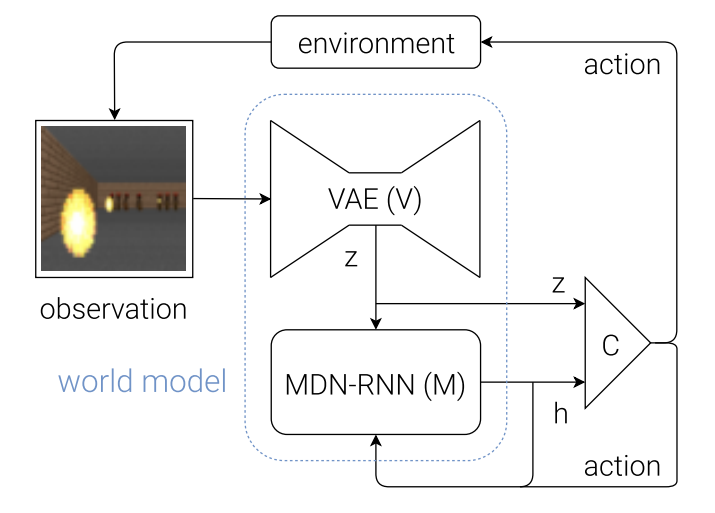
\includegraphics[width=.5\textwidth]{./world_model.png}
    \caption{In the World Model, the $z$ is produced by VAE, so $z$ is the parameters of some distributions.}
\end{figure}

Now if we look at it closely.
VAE assumes there is only one distribution: the Normal distributions.
Here, $z$ only contains $\mu$'s and $\sigma$'s.
What if we can have many different generative models, e.g. $z_1$, $z_2$, $z_3$, ... with different distributions?

Basically, we want to construct new VAE's, not only use the Normal distribution, but other distributions as well.
\cite{davidson_hyperspherical_2018} shows the Normal distribution can be replaced by a von Mises-Fisher (vMF) distribution, so the $\cal{S}$-VAE can better capture data with a hyperspherical latent structure.
Different models must have different abilities.
The original VAE paper \cite{kingma_auto-encoding_2014} also mentioned the probability of using other distributions.

But what distributions should be chosen to this fleet? It's not clear.
Maybe here we can apply Evolutionary Algorithms to get some better models.


\bibliographystyle{apalike}
\bibliography{b}

\end{document}
